% **************************************************************************** %
\chapter{\code{LTspice}-Schaltungen}
\label{app:ltspice}
% **************************************************************************** %

Dieses Kapitel  beinhaltet \code{LTspice}-Schaltungen, welche  zu Simulationen
benutzt  worden  sind. Erkl\"arungen zu  den  jeweiligen  Schaltungen sind  in
den  Kapiteln zu  finden, welche  auf  sie verweisen. Zu  jeder Schaltung  ist
angegeben, wo sie auf dem Datentr\"ager gefunden werden kann.

\noindent\begin{minipage}{\textwidth}
    \centering
    
\includegraphics[width=0.9\textwidth]{images/ltspice/generic-iv-curves/cell.eps}
    \figcaption[\code{LTspice}-Schaltung f\"ur PV-Zelle]{%
        Modell   der   PV-Zelle,   aus   welchem  das   Modul   in   Abbildung
        \ref{fig:ltspice:iv:generic:module}  aufgebaut  ist. Die  Simulationen
        aus   Abbildung   \ref{fig:simu:iv-curves:module:generic}  auf   Seite
        \pageref{fig:simu:iv-curves:module:generic}   basieren    auf   diesem
        Modell. Gegen\"uber   dem   in   Abschnitt   \ref{sec:simu:model:cell}
        hergeleiteten Modell hat dieses  Modell einen h\"oheren Photostrom und
        einen niedrigeren Shunt-Widerstand. Dies  erzeugt etwas anschaulichere
        Kurven.\protect\\
        Dateipfad: \code{ltspice/generic/cell-9A.asc}%
    }
    \label{fig:ltspice:iv:generic:cell}
    
\includegraphics[width=0.9\textwidth]{images/ltspice/jac/cell.eps}
    \figcaption[\code{LTspice}-Schaltung f\"ur PV-Zelle]{%
        Modell  der   PV-Zelle,  auf  welchen  die   Simulationen  in  Kapitel
        \ref{chap:simu} ab  Seite \pageref{chap:simu}  beruhen. Die Herleitung
        ist in Abschnitt \ref{sec:simu:model:cell} dokumentiert.\protect\\
        Dateipfad: \code{ltspice/jac/jac-cell.asc}%
    }
    \label{fig:ltspice:jac:cell}
\end{minipage}

\clearpage
\begin{figure}[h!tb]
    \centering
    \begin{tikzpicture}[%
        spy scope = {magnification=7,size=25*8,connect spies},
        every spy on node/.style={circle,red,draw},
        every spy in node/.style = {circle, fill=white, fill opacity=1, draw},
        ]
        \node[inner sep = 0pt,anchor=south west] {%
            
\includegraphics[width=\textwidth]{images/ltspice/generic-iv-curves/module.eps}
        };
        \spy[red] on (0.45,1.2) in node at (10,8);
    \end{tikzpicture}
    \caption[\code{LTspice}-Schaltung f\"ur PV-Modul f\"ur IV- und PV-Kurven]{%
        \code{LTspice}-Modell,    welches    zur    Erzeugung    der    Kurven
        in   Abbildung   \ref{fig:simu:iv-curves:module:generic}   auf   Seite
        \pageref{fig:simu:iv-curves:module:generic}  benutzt  worden  ist. Das
        Modell  der Zelle,  aus welcher  dieses  Modul aufgebaut  ist, ist  in
        Abbildung \ref{fig:ltspice:iv:generic:cell} abgebildet.\protect\\
        Dateipfad: \code{ltspice/generic/module-9A.asc}%
    }
    \label{fig:ltspice:iv:generic:module}
\end{figure}

\clearpage
Bei  \hfill Schaltungen  mit \hfill  hunderten oder  gar tausenden  \hfill von
Komponenten  wird\\ \code{LTspice}  sehr schwerf\"allig  zum Bedienen,  da das
Updaten der  Netlist sehr lange  dauert und  die Netlist bei  jeder \"Anderung
der  Schaltung  aktualisiert  werden  muss.  Zur  einfacheren  Handhabung  von
Simulationen  mit mehreren  Modulen wird  deshalb ein  neues Symbol  f\"ur ein
Modul definiert, gezeigt in Abbildung \ref{fig:ltspice:module:symbol}, welches
je nach Bedarf  mit der Schaltung f\"ur ein Modul  mit oder ohne Freilaufdiode
verkn\"upft werden kann.

\begin{figure}[h!tb]
    \centering
    
\includegraphics[width=0.4\textwidth]{images/ltspice/module-symbol.eps}
    \caption{%
        Selbst erstelltes Symbol f\"ur PV-Modul\protect\\
        Dateipfad:   \code{ltspice/jac/jacModule.asy}   (mit   Freilaufdioden,
        verkn\"upft          mit          Modul         aus          Abbildung
        \ref{fig:ltspice:jacModule:NoDiode})\protect\\
        Dateipfad: \code{ltspice/jac/jacModuleNoD.asy} (ohne Freilaufdioden, verknupft mit
        Modul aus Abbildung \ref{fig:ltspice:jacModule:Diode})%
    }
    \label{fig:ltspice:module:symbol}
\end{figure}

\begin{figure}[h!tb]
    \centering
    
\includegraphics[width=\textwidth]{images/ltspice/jac/stringNoD.eps}
    \caption[\code{LTspice}-Schaltung f\"ur Modulstrang]{%
        \code{LTspice}-Schaltung  f\"ur  einen   Modulstrang  aus  20  Modulen
        und   variablem  Lastwiderstand   \code{Rload}   zur  Erstellung   von
        Strom-Spannungs-Kurven. Es  wird   je  ein  Strang  aus   Modulen  mit
        Freilaufdiode   (Abbildung  \ref{fig:ltspice:jacModule:NoDiode})   und
        ohne   Freilaufdiode   (Abbildung   \ref{fig:ltspice:jacModule:Diode})
        simuliert.\protect\\
        Dateipfad: \code{ltspice/jac/string.asc} (mit Freilaufdioden)\protect\\
        Dateipfad: \code{ltspice/jac/stringNoD.asc} (ohne Freilaufdioden)%
    }
    \label{fig:ltspice:string:ivCurve}
\end{figure}

\begin{figure}[h!tb]
    \centering
    \begin{tikzpicture}[%
        spy scope = {magnification=5,height=25*5.5,width=25*10,connect spies},
        every spy on node/.style={rectangle,red,draw},
        every spy in node/.style = {rectangle,fill=white, fill opacity=1, draw},
        ]
        \node[inner sep = 0pt,anchor=south west] {%
            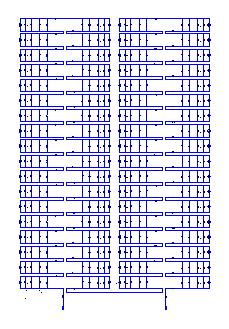
\includegraphics[width=\textwidth]{images/ltspice/jac/jacModuleNoD.eps}
        };
        \spy[red] on (1.15,1.13) in node at (9,8);
    \end{tikzpicture}
    \caption[\code{LTspice}-Schaltung f\"ur PV-Modul ohne Freilaufdiode]{%
        Modul    ohne   Freilaufdiode,    benutzt    f\"ur   die    Simulation
        aus   Abbildung   \ref{fig:simu:iv-curves:array:generic}   von   Seite
        \pageref{fig:simu:iv-curves:array:generic}.\protect\\
        Dateipfad: \code{ltspice/jac/jacModuleNoD.asc}%
    }
    \label{fig:ltspice:jacModule:NoDiode}
\end{figure}

\begin{figure}[h!tb]
    \centering
    \begin{tikzpicture}[%
        spy scope = {magnification=5,height=25*5.5,width=25*10,connect spies},
        every spy on node/.style={red,draw},
        every spy in node/.style = {fill=white, fill opacity=1, draw},
        ]
        \node[inner sep = 0pt,anchor=south west] {%
            \includegraphics[width=\textwidth]{images/ltspice/jac/jacModule.eps}
        };
        \spy[rectangle,red] on (1.15,1.13) in node at (9,8);
        \spy[circle,size=25*3,red] on (7.05,0.9) in node at (9,3);
    \end{tikzpicture}
    \caption[\code{LTspice}-Schaltung f\"ur PV-Modul mit Freilaufdiode]{%
        Modul      mit      Freilaufdiode       (unten,      Mitte,      Diode
        \code{D145}). Benutzt       f\"ur       die       Simulation       aus
        Abbildung   \ref{fig:simu:iv-curves:array:generic:bypass}  von   Seite
        \pageref{fig:simu:iv-curves:array:generic:bypass}       sowie      die
        Simulationen zu den L\"osungsvarianten in Abschnitt
        \ref{sec:simu:coupling:inductive} ab Seite
        \pageref{sec:simu:coupling:inductive}, Abschnitt
        \ref{sec:simu:coupling:capacitive} ab Seite
        \pageref{sec:simu:coupling:capacitive} und Abschnitt
        \ref{sec:simu:short} ab Seite
        \pageref{sec:simu:short}.
        Abbildung   \ref{fig:ltspice:jac:cell}    enth\"alt   das   verwendete
        Zellenmodell.\protect\\
        Dateipfad: \code{ltspice/jac/jacModule.asc}%
    }
    \label{fig:ltspice:jacModule:Diode}
\end{figure}
